\chapter{Transportation planning problems}

In this chapter, we formalize the concept of planning to help us with formally introducing the studied transportation problems. We will also formalize the Transport domain and mention similar problems that have been studied.

\section{Automated planning}

As previously stated, \textit{planning} is usually defined as the reasoning side of acting --- an abstract deliberation
process that chooses and organizes actions by anticipating their outcomes. \citep[Section~1.1]{Ghallab2004}
It seems only natural that we want to have computers do this strenuous activity for us.
Automated planning is an attempt at just that --- it is an area of Artificial Intelligence (AI) that
studies the planning process computationally. \citep[Section~1.1]{Ghallab2004}

Unfortunately, the specific situations in which we want to use automated planning are very diverse
--- from devising a sequence of actions to shut down a nuclear power plant,
planning the movements of a robotic arm
on an assembly line, or devising the complex pattern of motor activations
for space aircraft positioning.
Due to this, researchers are often interested in domain-independent planning,
where the planner gets information
about both the domain and the specific problem at runtime and attempts to devise a plan using only the provided knowledge
and the planner's previously built-in processes. \citep[Section~1.3]{Ghallab2004}

On the other hand, domain-specific planning, where domain knowledge has been built into the planner,
has obvious advantages when solving problems in that domain --- all the while being useless on problems of other
domains. \citep[Section~1.3]{Ghallab2004}

\subsection{Planning model}

As a basis for the later-defined representation of planning, we first define
a conceptual model similar to the restricted model in \citep[Section~1.4, Section~1.5]{Ghallab2004}.

\begin{defn}[State-transition system]\label{defn:state-transition-sys}
A (restricted) state-transition system is a 3-tuple $\Sigma = (S, A, \gamma)$, where:
\begin{itemize}
\item $S = \{s_1, s_2, \ldots\}$ is a finite and fully observable set of states;
\item $A = \{\noop, a_1, a_2, \ldots\}$ is a finite set of actions;
\item $\gamma: S \times A \to S \cup \{\emptyset\}$ is a state-transition function,
where $\forall s \in S : \gamma(s, \noop) = s$,
and $\forall s \in S\,\exists a \in A : \gamma(s, a) \neq \emptyset$; and
\item $\Sigma$ is static and offline,
it only changes when an action is applied to it and does not change while planning.
\end{itemize}
In the basic version, all actions have no duration.
\end{defn}

For a state $s \in S$, the actions $A_s = \{a \in A | \gamma(s, a) \neq \emptyset\}$ are called \textit{applicable}
to the given state $s$. The $\noop$ action is applicable to all states.

The state-transition function $\gamma$ and the set of actions $A$ together loosely correspond to what we will call a \textit{planning domain}.
Planning domains define an abstract representation of actions we work with
and how they are related,
but they do not state anything about specific states or actions.

Given a state-transition system $\Sigma$, planning aims to find a
sequence of actions to apply to the beginning state in order to achieve some objective.
The objective can be defined in various ways --- we might want the planner
to devise a plan that
does not enter specific states, or contrary to that, visits each of a set of states,
or one that just ends at a chosen state.
We will use the last option for formalizing the notion of a \textit{planning problem}.

\begin{defn}[Planning problem]\label{defn:planning-problem}\citep[Part~I]{Ghallab2004}
A planning problem is a 5-tuple $\mathcal{P} = (S, A, \gamma, s_0, g)$, where:
\begin{itemize}
\item $(S, A, \gamma)$ is a state-transition system;
\item $s_0 \in S$ is an initial state; and
\item $g \subseteq S$ is a set of goal states.
\end{itemize}
\end{defn}

Now that we have defined a \textit{planning problem} we can specify what we mean
by the planner generating a \textit{sequence of actions} to achieve a goal --- we will
call this sequence a \textit{plan}.

\begin{defn}[Plan]\label{defn:plan}\citep[Section~1.5]{Ghallab2004}
For a planning problem $\mathcal{P} = (S, A, \gamma, s_0, g)$,
a plan is a finite sequence of actions $(a_1, a_2, \ldots, a_k),\, k \in \N$ where
$\forall i \in \kset : a_i \in A$ and
$\forall i \in \kset : \gamma(s_{i-1}, a_i) = s_i \in S$, while $s_k \in g$.
\end{defn}

A basic \textit{planning model}, i.e. the abstraction of a whole real-life scenario
we want to plan for, consists of three components (Figure~\ref{fig:planning-model}):
\begin{itemize}
\item A \textit{state-transition system} $\Sigma$, that evolves by using its state-transition function on the actions
it receives;
\item A \textit{controller}, that given an input state $s \in S$ and a generated plan, provides an action $a \in A$ as output; and
\item A \textit{planner}, that uses a description of the state-transition system $\Sigma$ to synthesize a plan for the controller
to execute in order to reach a goal state from the initial state.
\end{itemize}

\begin{figure}[tb]
\begin{center}
\includegraphics[width=0.7\textwidth]{../imga/planning_model}
\end{center}
\caption[A typical planning model for offline planning.]{A typical planning model for offline planning --- a state-transition system $\Sigma$, a controller executing a plan, and a planner devising the plan based on an initial state and goals. Adapted from \citep[Figure~1.3]{Ghallab2004}.}
\label{fig:planning-model}
\end{figure}

\subsection{Classical planning}\label{classical-planning}

Although the previously defined restricted state-transition system is a simplification of real-world
domains, it is a useful one. 
This simplification has historically been studied as classical planning.

A different branch of automated planning, \textit{neoclassical planning},
uses largely the same theoretical foundations as classical 
planning. What is different is the approach to planning using those foundations
--- instead of search space nodes being a sequence of actions or a partially ordered
set of actions, we view them as a set of several partial plans
\citep[Part~II]{Ghallab2004}.
One of the most famous results in neoclassical planning is the GraphPlan algorithm
published by \citet{Blum1997}. It is out of the scope of this text to describe it in detail
--- see \citet[Section~6.3]{Ghallab2004}.
GraphPlan makes heavy use of a data structure called a \textit{planning graph},
which caused a breakthrough in the field of (domain-independent) planning
--- bigger problems could now be practically solved.

We will now describe several theoretical domain-independent representations
of planning problems used in classical planning \citep[Chapter~2]{Ghallab2004},
so that we can formulate our domain using them.

\subsubsection{Set-theoretic representation}

Leveraging propositional logic, both the planning domain and problem
are represented with the notion
of proposition symbols $L = \{p_1, p_2, \ldots\}$.
Each state is defined as a subset of propositions of $L$ --- those propositions
which hold in the given state. $S$ is closed under the application of each
action $a \in A$.

An action $a$
is a triple of sets of propositions of $L$.
We denote the sets $a = (\precond(a), \effects^-(a), \effects^+(a))$, where:
\begin{itemize}
\item $\precond(a)$ are the \textit{preconditions} of an action: the set of
propositions that must hold in the current state for the action to be applicable to it;
\item $\effects^-(a)$ are the \textit{negative effects} of an action:
the set of propositions
that will no longer hold in the state once the action is applied; and
\item similarly, $\effects^+(a)$ are the \textit{positive effects} of an action:
the set of propositions that will be true in the state once the action is applied.
\end{itemize}

The state-transition function is $\gamma(s, a) = (s - \effects^-(a)) \,\cup\,
\effects^+(a)$ if $a$ is applicable to $s$,
otherwise $\gamma(s, a)$ is undefined. Goal states $S_g$ are defined as
$S_g = \{s \in S \,|\, g \subseteq s\}$, where
$g \subseteq L$ is any chosen set of propositions. The propositions $g$ are called
\textit{goal propositions}.

\subsubsection{Classical representation}

The classical representation generalizes the set-theoretic representation using first-order logic,
without functions.
States are sets of ground atoms of a first-order language.
Actions are ground instances of \textit{planning operators},
triples $o = (\name(o), \precond(o), \effects(o))$:

\begin{itemize}
\item $\name(o)$ is a syntactic expression of the given operator;
\item $\precond(o)$ and $\effects(o)$ are sets of literals
(atoms and their negations), similar in use to their equivalents
in the set-theoretic case.
\end{itemize}

The definition of the state-transition function also stays the same.
Goal states are defined as the set of states that satisfy $g$,
the \textit{goal}, where $g$ is any set of ground literals.

Both the set-theoretic and the classical representations follow the \textit{Closed world assumption} --- that any atom/predicate not present in the state does not hold in that state.

\subsubsection{State-variable representation}

The state-variable representation substitutes the use of relations of the previous
representation for functions,
using the concept of state variables. State variables are functions
that take the state as an input and serve as characteristic attributes, defining the state. We usually use a more practical way of defining these functions --- we assume
the current state as an input without denoting it, and instead add different inputs.

For example, a useful set of state-variable functions for a domain that contains a road
network and vehicles might be: $$\mathrm{location}_{v}: S \to \mathrm{locations},$$
where $v \in \mathrm{vehicles}$.
Instead, we could define a single function:
$$\mathrm{location'}: \mathrm{vehicles} \times S \to \mathrm{locations},$$
and afterwards 
$$\mathrm{location''}: \mathrm{vehicles} \to \mathrm{locations},$$
using $\mathrm{location''}(v) = \mathrm{location'}(v, state_{cur})$, where $state_{cur}$ is the current state.

Planning operators are defined similarly to the classical representation, but
$\precond(o)$ is now a set of expressions on state variables and relations.
Also, $\effects(o)$ is defined as a set of assignments of values to state variables.
The state-transition function is defined analogously: an action $a$ (ground instance
of operator $o$)
is applicable to a state $s$ if the $\precond(o)$ condition is true given the values
of state variables in state $s$. The resulting state is created by changing the state variables
according to the assignments in $\effects(o)$ and the corresponding values of state
variables in state $s$.
The goal is defined as a set of ground state variables and their corresponding values
\citep[Section~2.5.2]{Ghallab2004}.


\subsubsection{Extensions of representations}

We will later extend these representations using types.
To see how types fit into our previously defined representations, we can
define a \textit{type} as a unary predicate, which has the value true
if and only if the predicate's argument is of the given type.
We can then add these predicates as preconditions of actions.
Adding types will make the domain and problem formulations
easier to read and gives additional information
to planners, making them more efficient \citep[Section 2.4.1]{Ghallab2004}.

\subsubsection{State-space planning and Plan-space planning}

A different way of viewing the state-transition system $\Sigma = (S, A, \gamma)$ in a
planning problem $\mathcal{P} = (S, A, \gamma, s_0, g)$ (Definition~\ref{defn:state-transition-sys}~and~\ref{defn:planning-problem}), is that of a labeled, directed graph $G(S, E, w)$, where:
\begin{itemize}
\item $E = \{(u, v) \in S^2 \;|\; \exists a \in A : \; \gamma(u, a) = v\}$;
\item $w: E \to A$; and
\item $\forall (u, v) = e \in E : w(e) = \{a \in A \;|\; \gamma(u, a) = v\}$. 
\end{itemize}
From the definition above, we see that applicable actions correspond to state transitions. While planning, the plan represented by the current position in
the state space is the sequence of transitions from the start
state $s_0$ to the current state \citep[Section~4.1]{Ghallab2004}.
\textit{State-space planning} is a term used for planning techniques
that use the state space for searching for a plan.

An alternative for using the state space is offered by \textit{plan-space planning}.
The state space is substituted for the \textit{plan space}.
Nodes in this space represent \textit{partially specified plans},
edges are \textit{plan refinement operations} \citep[Section~5.1]{Ghallab2004}.
We will not use plan-space planning in this work, as according to
\citet[Section~5.6]{Ghallab2004} it is unfit for
incorporating domain-specific knowledge.

\subsubsection{Temporal planning}

The addition of time makes modeling planning problems difficult and
solving them even more difficult.
However, adding time makes most models more realistic and practically usable.

For an exhaustive introduction to temporal planning, see \citet[Chapter~13~and~14]{Ghallab2004}. We will only use the \textit{durative action} modeling approach
specified by \citet[Section~5]{Fox2003}. We will adapt the following concepts presented
in \citet[Section~14.2]{Ghallab2004} that are relevant to modeling temporal transportation planning problems:
\begin{itemize}
\item A \textit{temporally qualified expression} (tqe) is any
expression in the form $$p(x_1, x_2, \ldots, x_k)@[t_s, t_e),$$ where $p$
is a relation of the planning domain and $x_1, \ldots, x_k$ are constants or \textit{object
variables}. These are similar to state variables in the state-variable representation,
but the values change in time, not between states).

The temporal variables $t_s$ and $t_e$ do not specifically represent a numerical time value, but together with other variables and constraints form a consistent set (for a more precise definition, see \citet[Section~14.2.1]{Ghallab2004}).
It holds that $t_s < t_e$.

The tqe $p(x_1, \ldots, x_k)@[t_s, t_e)$
asserts that the relation $p(x_1, \ldots, x_k)$ holds for any time $t$, where
$t_s \leq t < t_e$.

\item A \textit{temporal planning operator} is a tuple $o$, defined similarly to the planning operator in classical representations, but $\precond(o)$ and $\effects(o)$ are tqes.
\end{itemize}



\subsection{PDDL}\label{pddl}

Originally proposed by \citet{McDermott1998} for the 1$^{\mathrm{st}}$ International Planning
Competition,\footnote{\url{http://ipc98.icaps-conference.org/}}
the Planning Domain Definition Language (PDDL) has become
a de facto standard language for modeling planning domains and problems,
continually evolving to the needs of the  
research community and the needs of the IPC itself in the future years.
We will also use it as input for our planners.

PDDL was inspired by the language used to describe STRIPS \citep{Fikes1971}
and the numerous languages that sparked from it.
It has a Lisp-like\footnote{\url{https://en.wikipedia.org/wiki/Lisp_(programming_language)}}
declarative syntax and is very extensible.
A basic (without using extensions) PDDL domain and problem definition essentially correspond to representation format of the already defined planning domains and problems. Confusingly, we call PDDL planning operators \textit{actions}.
Each action has a list of \textit{parameters} to be grounded by the planner,
a \textit{precondition} and an \textit{effect}. To denote multiple
preconditions and effects, we use the n-ary predicate \texttt{and}.
A full format specification applicable to our use case is available in \citet[Appendix A]{Fox2003}.

Not many planners support PDDL in its entirety --- they usually support 
several ``feature subsets'', called \textit{requirements}.
One problem with the diversity of these requirements is that rarely does
a single planner support more than a few, which makes comparing them on a diverse
set of problems difficult.

An important version of PDDL, version 2.1, added support for temporal
planning using \textit{durative actions} \citep[Section~5]{Fox2003},
an analog of the previously defined temporal planning operators.
Specifically, every durative action has a \texttt{duration}, specified
either by a constant or a numeric fluent (a function with numerical values that
can change over time). Also, instead of a precondition it introduces a \textit{condition} (it is not necessary that the condition takes place before the action).
We will only use so-called \textit{discretized} durative actions, meaning that both the condition and the effect represent a temporally qualified expression,
denoted using three unary PDDL predicates:
\begin{itemize}
\item \texttt{at start}, where the parameter predicate must hold or the parameter effect must be applied at the start of the action;
\item \texttt{at end}, where it must hold or be applied at the end of the action; and
\item \texttt{over all}, where the parameter must hold over the duration of the action, start and end non-inclusive. This temporal predicate is not applicable to effects, as it is unclear what it would mean.
\end{itemize}

Over time, PDDL has evolved from the originally proposed version 1.2
to the now standard version 3.1. Several extensions and successors were proposed,
like Multi-Agent PDDL\comment{\footnote{\url{http://agents.fel.cvut.cz/codmap/}}}
(MA-PDDL) and
Probabilistic PDDL\comment{\footnote{\url{http://www.tempastic.org/papers/CMU-CS-04-167.pdf}}}
(PPDDL).

PDDL does not specify a representation for plans. For a specific planning domain and problem in PDDL,
we represent the plan in a format that is a field-wide consensus --- we will refer to is
as the \textit{VAL-like} format. VAL \citep{Howey2003} is a plan validator created for the IPC.
It takes as input (among several options) three filenames: filename of a planning domain and
problem in PDDL, and a filename for a plan in the mentioned format.
As described in and around \citet[Figure~2]{Howey2003}, the approximate format
consists of multiple lines in the following format:
\begin{center}
\verb+(action_name action_object_literals*)+
\end{center}

For temporal domains, the format adds a start time and duration for each line, like so:
\begin{center}
\verb+start_time: (action_name action_object_literals*) [duration]+
\end{center}
Both \verb+start_time+ and \verb+duration+ are floating-point numbers, with a dot as a decimal delimiter.

Note that all text between a semicolon \verb+;+ and an end-of-line character sequence \verb+\r+, \verb+\n+, or \verb+\r\n+ is regarded as a comment and ignored by all parsers.

\subsection{Planning in practice}

In practice, many of the assumptions we made will get violated and many additional requirements will arise,
due to various business or social requirements.
These assumptions allow us, however, to work
on problems that are more general and can, therefore, be applied to multiple scenarios.
Businesses can often add minor tweaks on top of the obtained results so that
their needs are satisfied. 
For example, online planning can often be foregone for some form of \textit{windowed} planning,
where we plan a certain time window offline and move on to the next window,
repeating the process regularly.

Planners, in practice, are computer programs that are fed two files as input
--- the domain file and the problem file. After that, they proceed with their internal calculations
and upon finishing return a plan (or not). 
We can then evaluate the plan, see if it meets our criteria and, potentially,
execute it in the real world.

What we are missing from a bare plan is the allocation of specific resources.
\textit{Scheduling} addresses the problem of how to perform a given set of actions (a plan)
using a limited number of resources in a limited amount of time, and
that is crucial to practical usage of any plan \citep[Chapter~15]{Ghallab2004}.

In this text, we will only study the abstracted and simplified first part of this whole process
--- finding the ``best'' actions that lead to a specified goal.
















\section{Description of Transport domain variants}

Transport is a planning domain designed for
the International Planning
Competition\footnote{\url{http://www.icaps-conference.org/index.php/Main/Competitions}}
(IPC), which is part of the International Conference on Automated Planning and
Scheduling\footnote{\url{http://www.icaps-conference.org/index.php/Main/HomePage}} (ICAPS).
Originally, Transport appeared at 
IPC-6\footnote{\url{http://icaps-conference.org/ipc2008/deterministic/Domains.html}} which took place in 2008.
Since then, it has been used in two IPCs,
specifically IPC-7\footnote{\url{http://www.plg.inf.uc3m.es/ipc2011-deterministic/}} in 2011
and IPC-8\footnote{\url{https://helios.hud.ac.uk/scommv/IPC-14/}} in 2014.

There are a few basic formulations of the Transport domain family (i.e.~``similar'' Transport domain variants) which we will describe now.

\subsection{Common traits of Transport domains}

Transport is a logistics domain --- vehicles drive around on a (generally asymmetric) positively-weighted oriented graph, picking up and dropping packages along the way.
All vehicles have limited capacities (the sum of package sizes they can carry).
Picking up or dropping a package costs 1 unit. The cost of driving along a road is equal to the edge weight
(in other words, the road length).
The general goal is to minimize the \textit{total cost}
while delivering all packages to their destination, where
the total cost of a plan is defined as the sum of the costs of all actions in
the plan.

A few Transport problems also request that the trucks be positioned at certain
locations in the graph
after finishing their deliveries.

\subsection{Transport STRIPS}\label{transport-strips}

STRIPS, the Stanford Research Institute Problem Solver,
was a planner proposed in the 1970s by \citet{Fikes1971}.
The influence of STRIPS was, however, not only due to the planner,
but the language used to describe its inputs --- the planning operators and goals.
That is why we sometimes refer to classical planning (Section~\ref{classical-planning})
as STRIPS planning. For the purposes of this text, we will use these terms interchangeably.

In the STRIPS variant of the Transport domain,
all packages have a size of 1 and vehicles of a bounded capacity can drive around indefinitely
(there is no notion of fuel or anything similar). The only reason for them not to, is that
driving incurs a cost of its own, usually much larger than picking up or dropping off packages.
This being a classical STRIPS domain,
it does not assume time in any sense,
so actions have no duration and are applied one after the other, sequentially.

This formulation contains three basic planning operators:

\begin{itemize}
\item \drive{}, where a vehicle drives to an adjacent location
along a road that is connected to its current location;
\item \pickup{}, where a vehicle that is stationary at a location picks up a co-located package; and
\item \drop{}, where a stationary vehicle drops a package off at its location.
\end{itemize}

In all the datasets, this domain variant is denoted as \textit{Transport sequential}
or \textit{transport-strips} and we will alternate between these terms in this text. See Figure~\ref{fig:ipc08_seq-sat_p13} for a visual example.

\begin{figure}[tbp]
\begin{center}
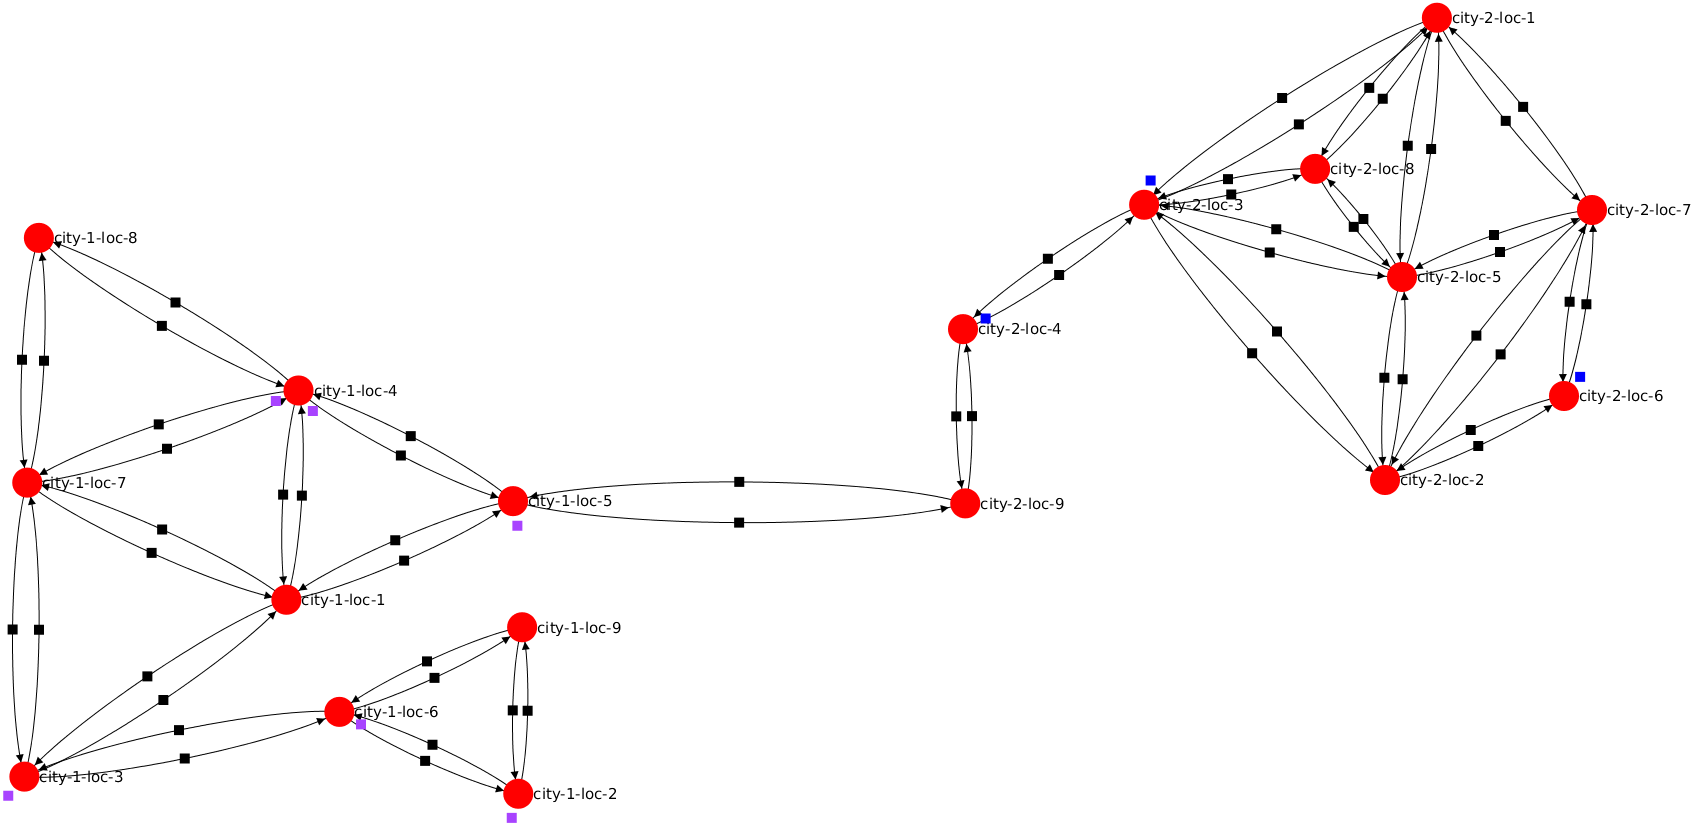
\includegraphics[width=1.0\textwidth]{../img/ipc08_seq-sat_p13_land2}
\end{center}
\caption[Visualization of the \texttt{p13} problem of sequential Transport from IPC 2008.]{Road graph visualization of the \texttt{p13} problem of the seq-sat track of IPC 2008. Red dots represent locations (graph nodes), roads (graph edges) are represented by black arrows, vehicles are plotted as blue squares, and packages as purple squares.}
\label{fig:ipc08_seq-sat_p13}
\end{figure}

\subsection{Transport Numeric}\label{transport-numeric}

The numeric variant adds the concept of fuel on top of the STRIPS variant.
All roads have an additional cost, called \verb+fuel-demand+, which is
subtracted from a vehicle's \verb+fuel-left+ value if it chooses to drive along that road.
Additionally, all vehicles have a maximum fuel capacity \verb+fuel-max+,
which they regain upon being the target of a \verb+refuel+ action. This action can only
be executed at a location that is marked as having a petrol station. Petrol stations
are static with respect to a given planning problem instance.

This variant is usually denoted as \textit{Transport numeric} or \textit{transport-numeric}.

\subsection{Transport Temporal}\label{transport-temporal}

The temporal Transport domain is usually denoted as \textit{Transport temporal} or, confusingly,
also \textit{transport-numeric}. A major difference with respect to the numeric variant is
the addition of time. All actions now have a duration (\verb+pick-up+ and \verb+drop+ both have a
duration of 1, \verb+refuel+ has a duration of 10, and the duration of \verb+drive+ is
equal to the length of the road we are driving along). Furthermore, packages can now have any integral size.

The addition of time poses numerous technical complications when formalizing this variant
--- its PDDL (Section~\ref{pddl}) formulation significantly differs from the two previous ones, but only in technical details, not in objectives of the model.
One important technicality is that a vehicle cannot pick up or drop packages concurrently --- it always handles packages one at a time. Also, vehicles cannot do other actions during driving to another location (they are essentially placed ``off the graph'' for the duration of driving).

The overall goal remains largely the same (deliver packages to their destinations), but we no longer optimize the total cost. Instead, we now minimize the total duration of a plan,
defined as the maximum time when an action is still taking place.
In practice, this translates to minimizing maximum end time over all actions.



















\section{Formalizing the Transport domain}

We will now translate the informal description of the Transport domain from the previous section to the formal representations we defined in Section~\ref{classical-planning}. We will not formulate all the domain variants in all representations as
they are very much alike and not needed for the comprehension of the following chapters.

\subsection{Transport's classical representation}\label{transport-classical-representation}

We are now able to show the sequential Transport domain in one of the representations
previously defined, namely,
the classical representation (Figure~\ref{code:classical-strips}).
Note that this representation does not contain the notion of a \textit{total cost}
of a plan that we will optimize for later.
The predicates used are:
\begin{itemize}
\item \verb+at(o, l)+, the package or vehicle \verb+o+ is at the
location \verb+l+;
\item \verb+capacity(v, s)+, the vehicle \verb+v+ currently has \verb+s+ free space --- \verb+s+ is a variable for space literals, a set of literals denoting the amount of space (essentially interpretable as a finite set of integers);
\item \verb+capacity-predecessor(s1, s2)+, the space literal represented by \verb+s1+
is directly smaller than the literal represented by \verb+s2+;
\item \verb+in(p, v)+, the package \verb+p+ is in the vehicle \verb+v+;
\item \verb+road(l1, l2)+, the location \verb+l1+ is directly adjacent to the location
\verb+l2+ by a road; and
\item \verb+road-length(l1, l2)+, the driving distance between location \verb+l1+
and \verb+l2+. Does not change while planning.
\end{itemize}

\begin{figure}[tbp]
\begin{code}
drive(v, l1, l2)
  ;; vehicle v moves from location l1 to an adjacent location l2
  precond: at(v, l1), road(l1, l2)
  effects: not at(v, l1), at(v, l2)

pick-up(v, l, p, s1, s2)
  ;; vehicle v picks up package p at location l,
  ;; decreasing its capacity from s2 to s1
  precond: at(v, l), at(p, l), capacity-predecessor(s1, s2),
           capacity(v, s2)
  effects: not at(p, l), in(p, v), capacity(v, s1),
           not capacity(v, s2)
  
drop(v, l, p, s1, s2)
  ;; vehicle v drops package p at location l,
  ;; increasing its capacity from s1 to s2
  precond: at(v, l), in(p, v), capacity-predecessor(s1, s2),
           capacity(v, s1)
  effects: not in(p, v), at(p, l), capacity(v, s2),
           not capacity(v, s1)
\end{code}
\caption{Classical formulation of \texttt{transport-strips}.}
\label{code:classical-strips}
\end{figure}

The numeric variant  adds the \verb+refuel+ operator, changes the \verb+drive+
operator, and adds a new fuel-related predicate \verb+has-petrol-station(l)+, that is true when the given location \verb+l+ has
a petrol station.
To model fuel, we need the addition of a few functions, namely:

\begin{itemize}
\item \verb+fuel-demand(l1, l2)+, the amount of fuel needed to drive
from location \verb+l1+ to location \verb+l2+;
\item \verb+fuel-left(v)+, the amount of fuel left in
the vehicle \verb+v+; and
\item \verb+fuel-max(v)+, the maximum amount of fuel
the vehicle \verb+v+ can contain, i.e. its fuel tank capacity.
\end{itemize}

It is obvious that we could substitute the functions for relations
and a finite amount of literals for any given problem instance of
the domain in this representation,
so that it adheres to the definition of a classical formulation.
For example, we could add literals representing a finite set of
natural numbers and predicate that represents
\verb+successor+ defined as $\texttt{successor}(a, b) \equiv a + 1 = b$.

We also abuse the notation with \verb+decrease+ and \verb+assign+;
the left parameter's value is to be decreased by the right
parameter's value or the left parameter's value is to be overridden
by the right parameter's value, respectively.

See Figure~\ref{code:classical-numeric} for the exact differences
in the representation after adding fuel.

\begin{figure}[tbp]
\begin{code}
drive(v, l1, l2)
  ;; vehicle v moves from location l1 to an adjacent location l2
  precond: at(v, l1), road(l1, l2), fuel-left(v) >= fuel-demand(l1, l2)
  effects: not at(v, l1), at(v, l2),
           decrease(fuel-left(v),  fuel-demand(l1, l2))
  
refuel(v, l)
  ;; vehicle v is refueled to the maximum at location l
  precond: at(v, l), has-petrol-station(l)
  effects: assign(fuel-left(v), fuel-max(v))
\end{code}
\caption[Partial classical formulation of \texttt{transport-numeric}.]{Classical formulation of \texttt{transport-numeric}'s differences compared to \texttt{transport-strips}.}
\label{code:classical-numeric}
\end{figure}

\subsection{Transport's state-variable representation}

We are now also able to show the sequential Transport domain
in the state-variable representation (Figure~\ref{code:statevar-strips}).
Some predicates (\verb+at+, \verb+capacity+ and \verb+in+) have been transformed
into state-variable functions with largely the same semantics as in
Section~\ref{transport-classical-representation}. Again, we leave out
the \textit{total cost} notion.

\begin{figure}[tbp]
\begin{code}
drive(v, l1, l2)
  ;; vehicle v moves from location l1 to an adjacent location l2
  precond: at(v) = l1, road(l1, l2)
  effects: at(v) <- l2

pick-up(v, l, p, s1, s2)
  ;; vehicle v picks up package p at location l,
  ;; decreasing its capacity from s2 to s1
  precond: at(v) = l, at(p) = l, s1 + 1 = s2, s2 > 0, capacity(v) = s2
  effects: at(p) <- nil, in(p) <- v, capacity(v) <- s1
  
drop(v, l, p, s1, s2)
  ;; vehicle v drops package p at location l,
  ;; increasing its capacity from s1 to s2
  precond: at(v) = l, in(p) = v, s1 = s2 - 1, capacity(v) = s1
  effects: in(p) <- nil, at(p) <- l, capacity(v) <- s2
\end{code}
\caption{State-variable formulation of \texttt{transport-strips}.}
\label{code:statevar-strips}
\end{figure}

The numeric variant again adds the \verb+refuel+ operator along with
a few fuel-related state-variable functions and predicates, and changes 
the \verb+drive+ operator (Figure~\ref{code:statevar-numeric}).

\begin{figure}[tb]
\begin{code}
drive(v, l1, l2)
  ;; vehicle v moves from location l1 to an adjacent location l2
  precond: at(v) = l1, road(l1, l2), fuel-left(v) >= fuel-demand(l1,l2)
  effects: at(v) <- l2, fuel-left(v) <- fuel-left(v)-fuel-demand(l1,l2)
  
refuel(v, l)
  ;; vehicle v is refueled to the maximum at location l
  precond: at(v) = l, has-petrol-station(l)
  effects: fuel-left(v) <- fuel-max(v)
\end{code}
\caption[Partial state-variable formulation of \texttt{transport-numeric}.]{State-variable formulation of \texttt{transport-numeric}'s differences
compared to \texttt{transport-strips}.}
\label{code:statevar-numeric}
\end{figure}

We will represent the temporal variant of Transport using a variant of the state-variable representation using temporal planning operators, further referred to as the \textit{temporal state-variable representation}.
On top of the fuel-related predicates and functions from \verb+transport-numeric+, temporal Transport adds:
\begin{itemize}
\item \verb+package-size(p)+, a function with positive integer values representing the size of the package \verb+p+ (does not change during planning); and
\item \verb+ready-loading(v)+, a predicate used for ``locking'' the vehicle \verb+v+ during \pickup{} and \drop{} actions (enforcing the property of these two actions happening sequentially in time for a given vehicle). It is important to note that the \refuel{} action does not
lock the vehicle, which means the vehicle can be refueled while dropping off and picking up packages.
\end{itemize}
Figure~\ref{code:statevar-temporal} shows the temporal state-variable representation of Transport temporal, using a shorter but clear notation.

\begin{figure}[tb]
\begin{code}
drive(v, l1, l2)
  ;; vehicle v moves from location l1 to an adjacent location l2
  duration: road-length(l1, l2)
  cond: (at(v) = l1)@s, (road(l1, l2))@s,
        (fuel-left(v) >= fuel-demand(l1, l2))@s
  effects: (at(v) != l1)@s, (at(v) = l2)@e,
           (fuel-left(v) <- fuel-left(v) - fuel-demand(l1, l2))@s

pick-up(v, l, p)
  ;; vehicle v picks up package p at location l
  duration: 1
  cond: (at(v) = l1)@[s, e), (at(p) = l1)@s, (ready-loading(v))@s,
        (capacity(v) >= package-size(p))@s
  effects: (at(p) = nil)@s, (in(p) = v)@e, (not ready-loading(v))@s,
           (capacity(v) <- capacity(v) - package-size(p))@s,
           (ready-loading(v))@e
  
drop(v, l, p)
  ;; vehicle v drops package p at location l
  duration: 1
  cond: (at(v) = l1)@[s, e), (in(p) = v)@s, (ready-loading(v))@s
  effects: (in(p) = nil)@s, (at(p) = l)@e, (not ready-loading(v))@s,
           (capacity(v) <- capacity(v) + package-size(p))@e,
           (ready-loading(v))@e
  
refuel(v, l)
  ;; vehicle v is refueled to the maximum at location l
  duration: 10
  cond: (at(v) = l1)@[s, e), (has-petrol-station(l))@s
  effects: (fuel-left(v) <- fuel-max(v))@e
\end{code}
\caption[State-variable formulation of temporal Transport.]{Temporal state-variable formulation of temporal Transport. The characters \texttt{s} and \texttt{e} represent the start and end temporal variables of the given action, respectively.}
\label{code:statevar-temporal}
\end{figure}

\subsection{PDDL formulation of Transport}

All formulations of the Transport domain use PDDL (Section~\ref{pddl}) version 2.1,
with the requirement \verb+typing+, which adds the notion of types for individual
literals. We will call these literals \textit{action objects}.

The STRIPS variant additionally needs \verb+action-costs+, a requirement adding
integer costs to individual planning operators. These costs may be constant
(like the ones for \verb+pick-up+, \verb+drop+ or \verb+refuel+),
or they may be dependent on the parameters of the instantiated operator (like
the cost of \verb+drive+).
The numeric variant
requires \verb+numeric-fluents+, which introduces native PDDL support for functions whose values correspond to numbers and can change over time. It also requires are
\verb+goal-utilities+, used for custom optimization functions and optional goal predicates.
The temporal domain is similar in requirements to the numeric one, except for
substituting \verb+goal-utilities+ for \verb+durative-actions+ (introduces time
and the duration of actions).
For reference, we will now show the PDDL representation of the sequential and temporal variant of
the Transport domain in Figure~\ref{code:pddl-strips} and Figure~\ref{code:pddl-temporal} respectively.

\begin{figure}[tbp]
\begin{code}
(:action drive
  :parameters (?v - vehicle ?l1 ?l2 - location)
  :precondition (and
      (at ?v ?l1)
      (road ?l1 ?l2))
  :effect (and
      (not (at ?v ?l1))
      (at ?v ?l2)
      (increase (total-cost) (road-length ?l1 ?l2))))
(:action pick-up
  :parameters (?v - vehicle ?l - location ?p - package
               ?s1 ?s2 - capacity-number)
  :precondition (and
      (at ?v ?l)
      (at ?p ?l)
      (capacity-predecessor ?s1 ?s2)
      (capacity ?v ?s2))
  :effect (and
      (not (at ?p ?l))
      (in ?p ?v)
      (capacity ?v ?s1)
      (not (capacity ?v ?s2))
      (increase (total-cost) 1)))
(:action drop
  :parameters (?v - vehicle ?l - location ?p - package
               ?s1 ?s2 - capacity-number)
  :precondition (and
      (at ?v ?l)
      (in ?p ?v)
      (capacity-predecessor ?s1 ?s2)
      (capacity ?v ?s1))
  :effect (and
      (not (in ?p ?v))
      (at ?p ?l)
      (capacity ?v ?s2)
      (not (capacity ?v ?s1))
      (increase (total-cost) 1)))
\end{code}
\caption{Formulation of actions in PDDL for \texttt{transport-strips}.}
\label{code:pddl-strips}
\end{figure}

\begin{figure}[tbp]
\begin{code}
(:durative-action drive
  :parameters (?v - vehicle ?l1 ?l2 - location)
  :duration (= ?duration (road-length ?l1 ?l2))
  :condition (and
      (at start (at ?v ?l1))
      (at start (road ?l1 ?l2))
      (at start (>= (fuel-left ?v) (fuel-demand ?l1 ?l2))))
  :effect (and
      (at start (not (at ?v ?l1)))
      (at end (at ?v ?l2))
      (at start (decrease (fuel-left ?v) (fuel-demand ?l1 ?l2)))))
(:durative-action pick-up
  :parameters (?v - vehicle ?l - location ?p - package)
  :duration (= ?duration 1)
  :condition (and
      (at start (at ?v ?l))
      (over all (at ?v ?l))
      (at start (at ?p ?l))
      (at start (>= (capacity ?v) (package-size ?p)))
      (at start (ready-loading ?v)))
  :effect (and
      (at start (not (at ?p ?l)))
      (at end (in ?p ?v))
      (at start (decrease (capacity ?v) (package-size ?p)))
      (at start (not (ready-loading ?v))) ; lock vehicle
      (at end (ready-loading ?v)))) ; unlock vehicle
(:durative-action drop
  :parameters (?v - vehicle ?l - location ?p - package)
  :duration (= ?duration 1)
  :condition (and
      (at start (at ?v ?l))
      (over all (at ?v ?l))   
      (at start (in ?p ?v))
      (at start (ready-loading ?v)))
  :effect (and (at start (not (in ?p ?v)))
      (at end (at ?p ?l))
      (at end (increase (capacity ?v) (package-size ?p)))
      (at start (not (ready-loading ?v))) ; lock vehicle
      (at end (ready-loading ?v)))) ; unlock vehicle
(:durative-action refuel
  :parameters (?v - vehicle ?l - location)
  :duration (= ?duration 10)
  :condition (and
      (at start (at ?v ?l))
      (over all (at ?v ?l))
      (at start (has-petrol-station ?l)))
  :effect
      (at end (assign (fuel-left ?v) (fuel-max ?v))))
\end{code}
\caption{Formulation of durative actions in PDDL for temporal Transport.}
\label{code:pddl-temporal}
\end{figure}
















\section{Related problems}

To the best of our knowledge, there has been no attempt at producing domain-dependent planners
for Transport (IPC 2008, 2011, 2014 and unsolvability IPC 2016) or any other similar IPC domain, like Logistics (IPC 1998\comment{\footnote{\url{https://web.archive.org/web/20151017170331/http://ipc98.icaps-conference.org/}}} and 2000),
Depots (IPC 2002\comment{\footnote{\url{https://web.archive.org/web/20170408120817/http://ipc02.icaps-conference.org/domains.html}}}),
DriverLog (IPC 2002 and 2014),
or Trucks (IPC 2006).
All techniques we know of applied to Transport so far are the
domain-independent planners used in the three before-mentioned competitions.

Most of the research done on transportation-related problems and their automation
generally focuses
on a famous combinatorial optimization problem, the \textit{Traveling Salesman Problem} (TSP), on which an
exhaustive amount of research has been done \citep{Applegate1998, Applegate2011}. Its precise origins are unknown, but the problem has been on the minds of researchers at least since the end of the 19$^\textrm{th}$ century. The TSP is defined by \citet{Applegate2011} as follows:
\begin{quote}
Given a set of cities along with the cost of travel between each pair of them, the \textit{traveling salesman problem}, or \textit{TSP} for short, is to find the cheapest way of visiting all the cities and returning to the starting point. The ``way of visiting all the cities'' is simply the order in which the cities are visited; the ordering is called a \textit{tour} or \textit{circuit} through the cities.
\end{quote}
However, the problem we aim to study is more similar to a different optimization problem based on the TSP. See Figure~\ref{fig:tsp} for an illustrative example of a TSP solution.

\begin{figure}[tbp]
\begin{center}
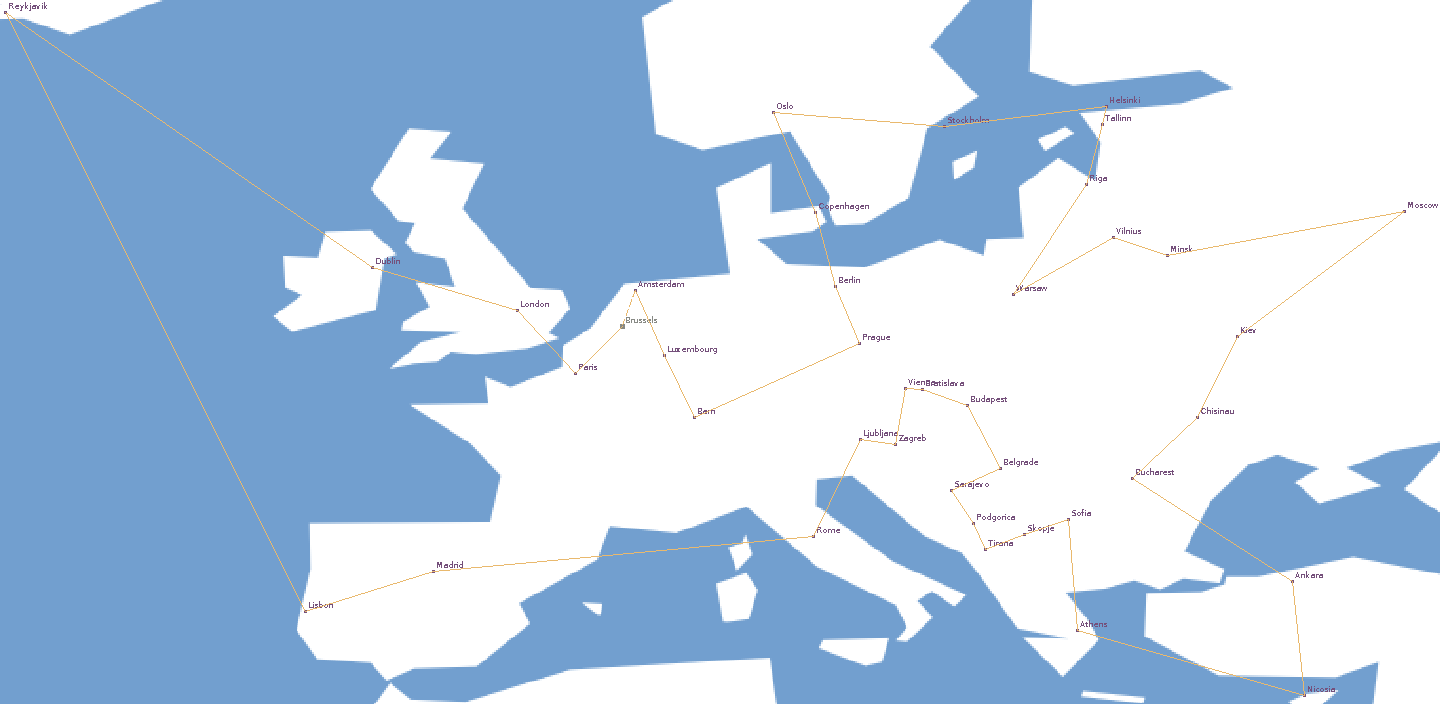
\includegraphics[width=1.0\textwidth]{../img/tsp}
\end{center}
\caption[An example TSP solution through cities in Europe.]{An example TSP solution through cities in Europe. Screenshot taken from OptaPlanner \citep{DeSmet2017}.}
\label{fig:tsp}
\end{figure}

\subsection{The Vehicle Routing Problem}\label{vrp}

The \textit{Vehicle Routing Problem} (VRP) was first formulated as the \textit{Truck Dispatching Problem} by \citet{Dantzig1959}, modeling a fleet of vehicles delivering gasoline to service stations. They described VRP
as a generalization of the TSP with multiple vehicles, but it could equivalently be stated that the TSP is a specialization of the VRP
with a single vehicle. The precise formulation of the Truck Dispatching Problem in \citep[Section~2]{Dantzig1959} represents a model with a fleet of identical vehicles departing from a single depot. According to \citet[Section~3]{Braekers2016}, this defines what we would call \textit{Capacitated VRP} (CVRP) today (Figure~\ref{fig:vrp}).

\begin{figure}[tbp]
\begin{center}
\includegraphics[width=0.7\textwidth]{../img/vrp}
\end{center}
\caption[An example CVRP solution for 32 customers and one depot.]{An example CVRP solution for 32 customers and one depot. Screenshot taken from OptaPlanner \citep{DeSmet2017}.}
\label{fig:vrp}
\end{figure}

Many VRP variants have emerged since. \citet{Eksioglu2009} and \citet{Braekers2016} both
review and classify hundreds of papers related to the VRP, with many more left out.
Most of these works tend to study the CVRP problem with minor modifications, hence creating
a broad landscape of problems and a platform to build on for the future.
According to the data in \citet[Table~4]{Braekers2016}, there has been a recent uptick
in popularity for models relatively similar to Transport --- specifically, VRPs with
backhauls (returning items from customers to depots),
multiple depots (multiple starting points for vehicles), and with allowed split deliveries (multiple
vehicles can serve a single customer).
The literature review on multiple depot VRP (MDVRP) in \citet{Montoya-Torres2015}
suggests a big rise in popularity for MDVRP in the recent past,
which provides further proof of relevance for studying the Transport domain.

Traditional solutions for the VRP include exact approaches like branch and bound
exploring the whole feasible search space,
classical heuristics which limit the search space, and also metaheuristics (general heuristics for devising specific heuristics), like genetic algorithms, constraint satisfaction
programming, local search, tabu search, and many more.

\comment{
\subsection{VRP Formulation}\citep{ResearchGroup2013}

The VRP is a combinatorial problem whose ground set is the edges of a graph ${G(V,E)}$. The notation used for this problem is as follows:

\begin{itemize}
\item ${V = \left\lbrace v_{0}, v_{1}, \ldots, v_{n} \right\rbrace}$ is a vertex set, where:
\begin{itemize}
\item Consider a depot to be located at ${v_0}$.
\item Let ${V' = V \backslash \left\lbrace v_{0} \right\rbrace}$ be used as the set of ${n}$ cities.
\end{itemize}
\item ${A = \left\lbrace(v_{i},v_{j}) | v_{i},v_{j} \in V; i \neq j \right\rbrace}$ is an arc set.
\item ${C}$ is a matrix of non-negative costs or distances ${c_{ij}}$ between customers ${v_{i}}$ and ${v_{j}}$.
\item ${d}$ is a vector of the customer demands.
\item ${R_{i}}$ is the route for vehicle ${i}$.
\item ${m}$ is the number of vehicles (all identical). One route is assigned to each vehicle.
\end{itemize}

When $c_{ij} = c_{ji}$ for all $(v_{i}, v_{j}) \in A$ the problem is said to be symmetric and it is then common to replace ${A}$ with the edge set $E = \lbrace (v_{i},v_{j}) | v_{i},v_{j} \in V; i < j \rbrace$.

With each vertex ${v_{i}}$ in ${V'}$ is associated a quantity ${q_{i}}$ of some goods to be delivered by a vehicle. The VRP thus consists of determining a set of ${m}$ vehicle routes of minimal total cost, starting and ending at a depot, such that every vertex in ${V'}$ is visited exactly once by one vehicle.

For easy computation, it can be defined ${b(V) = \left\lceil \sum_{v_{i} \in V} d_{i}) / C \right\rceil}$, an obvious lower bound on the number of trucks needed to service the customers in set ${V}$.

We will consider a service time $\delta_{i}$ (time needed to unload all goods), required by a vehicle to unload the quantity ${q_{i}}$ at ${v_{i}}$. It is required that the total duration of any vehicle route (travel plus service times) may not surpass a given bound ${D}$, so, in this context the cost ${c_{ij}}$ is taken to be the travel time between the cities. The VRP defined above is NP-hard [Lenstra \& Rinnooy Kan 1981].

A feasible solution is composed of:

\begin{itemize}
\item a partition ${R_{1}, \ldots, R_{m}}$ of ${V}$;
\item a permutation ${\sigma_{i}}$ of ${R_{i} \bigcup {0}}$ specifying the order of the customers on route ${i}$.
\end{itemize}


The cost of a given route (${R_{i} = \left\lbrace v_{0}, v_{1}, \ldots, v_{m+1} \right\rbrace}$), where ${v_{i} \in V}$ and ${v_{0} = v_{m+1} = 0}$ (0 denotes the depot), is given by ${C(R_{i}) = \sum_{i=0}^{m} c_{i,i+1} + \sum_{i=1}^{m} \delta_{i}}$.

A route ${R_{i}}$ is feasible if the vehicle stop exactly once in each customer and the total duration of the route does not exceed a prespecified bound ${D}$: ${C(R_{i}) \leq D}$.

Finally, the cost of the problem solution ${S}$ is: ${F_{VRP} = \sum_{i=1}^{m} F(R_{i})}$.
}

\subsection{Comparison of Transport and VRP}

In \citet{ResearchGroup2013}, a website was created, which serves as a comprehensive resource on the history of VRP,
definitions of its various flavors, and an overview of the popular solution methods and state-of-the-art results. According to the taxonomy they propose, we could characterize a Transport domain problem
as a \textit{Multiple Depot, Split Delivery, Capacitated VRP with Satellite Facilities}. Multiple Depot
means that vehicles can start driving from multiple locations, split delivery
means a single customer can be served by multiple vehicles, capacitated VRP adds maximum
capacities to vehicles, and satellite facilities mean that vehicles can pick items up
while on a delivery route. This does not characterize the Transport domain in every detail, but it is a fairly accurate approximation.

According to another VRP taxonomy and study of papers, presented in \citet{Eksioglu2009} and adapted in \citet{Braekers2016}, no research has been done on a VRP variant with a similar subset of features to those of Transport in any single study, to the best of our knowledge.
Usually, the studied problems are more constrained than Transport --- for example, they make additional assumptions about the places where vehicles start or end. Also, VRP in general
makes cooperation of vehicles hard to model, whereas in Transport this is one of the fundamental elements.

\comment{Transport could be characterized as \textit{2.1.1, 2.2.1, 2.4.1, 2.5.1, 2.8.1, 3.1.1, 3.2.2, 3.3.3, 3.4.2, 3.5.2, 3.7.1, 3.8.1, 3.9.3, 3.10.1, 3.11.1, 4.1.1, 4.2.1, 4.3.2, 4.4.1, 5.1.2.}}

An important difference between Transport and the VRP is that Transport has a notion of single packages or items. In the VRP, transported goods are usually regarded as measurable, rather than countable (for example gasoline or milk vs. letters or parcels). This makes a difference not only in the
interpretation, but also during problem-solving --- \textit{customers} in VRP usually request
a quantity of the delivered item, not specific item instances, like packages being ``requested''
by their target locations in Transport.

\subsection{Constraint Satisfaction Problems}\label{csp}

Constraint satisfaction techniques are a popular means of solving problems in combinatorial optimization. \citet[Section~8.1]{Ghallab2004} give an informal definition of a
\textit{Constraint Satisfaction Problem} (CSP):
\begin{quote}
Given (1) a set of variables and their respective domains, and (2) a set of constraints on the compatible values that the variables may take, the problem is to find a value for each variable within its domain such that these values meet all the constraints.
\end{quote}

We define the \textit{state space} of a CSP as all the possible combinations of assignments of values to the variables, respecting the domains of variables.
The size of the state space is simply the number of those combinations.

For example, the famous $n$-queens problem, where the goal is to position $n$ chess-style queen pieces on an $n \times n$ sized chessboard so that they do not attack each other (according to the rules of chess). Using a simple invariant deduced from the constraints (each queen has to occupy a different column),
we can model the problem as a CSP with $n$-ary variables $C_i \in [n]\; \forall i \in [n]$, one variable for each of the $n$ columns. The value of $C_i$ then represents the row the queen in column $i$ occupies. This problem has a search space size of $\prod_{i=1}^n n = n^n$, because any of the $n$ queens can be placed on any of the $n$ squares in its column \citep{Russell1995}.

We will attempt to model Transport as a CSP later on in Section~\ref{csp-formulation}.
Note that the translation of a VRP into a CSP representation is very natural and straightforward \citep[Solution Methods / Constraint Programming]{ResearchGroup2013}, which is usually not the case for planning problems.
